\begin{dang}{Các bài toán thực tế}
	
\end{dang}

\begin{vd}%[1K7KO-8]
	\immini{
		Hai mái nhà trong hình bên là hai hình chữ nhật ($AOPD$ và $BOPC$). Giả sử $AB=4{,}8\mathrm{~m}$, $OA=2{,}8 \mathrm{~m}$, $OB=4\mathrm{~m}$.
	}{
		\begin{tikzpicture}[scale=0.7, font=\footnotesize, line join=round, line cap=round, >=stealth]
			\path 
			(0,0) coordinate (P)
			(-2,-1.5) coordinate (D)
			(1,-1) coordinate (C)
			(5,0) coordinate (x);
			%	\tkzDefPoints{0/0/P,-2/-1.5/D,1/-1/C,5/0/x}
			\coordinate (O) at ($(P)+(x)$);
			\coordinate (A) at ($(D)+(x)$);
			\coordinate (B) at ($(C)+(x)$);
			\draw (A)--(B)--(O)--(P)--(D)--(A)--(O);
			\draw[dashed] (P)--(C)--(D) (B)--(C);
			%	\tkzDrawSegments(P,D O,A O,B A,B P,O D,A)
			%	\tkzDrawSegments[dashed](B,C C,D P,C)
			\foreach \x/\g in {A/-120,B/45,O/90,P/90,D/-120,C/45} \fill[black] (\x) circle (1pt) +(\g:0.3)node{$\x$};
		\end{tikzpicture}
	}
	\begin{enumerate}
		\item Tính (gần đúng) số đo của góc nhị diện tạo bởi hai nửa mặt phẳng tương ứng chứa hai mái nhà.
		\item Chứng minh rằng mặt phẳng $(OAB)$ vuông góc với mặt đất phẳng. Lưu ý: Đường giao giữa hai mái (đường nóc) song song với mặt đất.
		\item Điểm $A$ ở độ cao (so với mặt đất) hơn điểm $B$ là $0{,}5 \mathrm{~m}$. Tính (gần đúng) góc giữa mái nhà (chứa $OB$) so với mặt đất.
	\end{enumerate}
	\loigiai{
		\begin{enumerate}
			\item Ta có $\heva{& AO\perp PO \\ & BO\perp PO}$ nên $\widehat{AOB}$ là một góc phẳng của góc nhị diện $[A,PO,B]$.\\
			Theo định lí cos, ta có
			\[\cos\widehat{AOB}=\dfrac{OA^2+OB^2-AB^2}{2\cdot OA\cdot OB}=\dfrac{2{,}8^2+4^2-4{,}8^2}{2\cdot 2{,}8\cdot 4}=\dfrac{1}{28}.\]
			Suy ra $\widehat{AOB}\approx 88^\circ$.
			
			\item Theo chứng minh trên, ta có $PO\perp (OAB)$.\\
			Mà $PO$ song với mặt đất nên $(OAB)$ vuông góc với mặt đất phẳng.
			
			\item Gọi $H$ là giao điểm của phương thẳng đứng đi qua $A$ và phương ngang đi qua $B$.
			\immini{
				Theo giả thiết, $AH=0{,}5$ m.\\
				Góc giữa mái nhà chứa $OB$ so với mặt đất chính là góc $\widehat{OBH}$.\\
				Ta có $\sin\widehat{ABH}=\dfrac{AH}{AB}=\dfrac{0{,}5}{4{,}8}=\dfrac{5}{48}$.\\
				Suy ra $\widehat{ABH}\approx 5{,}98^\circ$.\\
				Theo định lí cos, ta có
			}{
				\begin{tikzpicture}[scale=1, font=\footnotesize, line join=round, line cap=round, >=stealth]
					\path 
					(0,0) coordinate (A)
					(2,2) coordinate (O)
					(5,-1) coordinate (B);
					%	\tkzDefPoints{0/0/A,2/2/O,5/-1/B}
					\coordinate (a) at ($(A)+(0,-2)$);
					\coordinate (H) at ($(A)!(B)!(a)$);
					\draw (A)--(O)--(B)--(A);
					%	\tkzDrawSegments(O,A O,B A,B)
					\draw[dashed] (A)--(H)--(B);
					\foreach \x/\g in {A/180,B/9,O/90,H/180} \fill[black] (\x) circle (1pt) +(\g:0.4)node{$\x$};
					%	\tkzMarkRightAngle(A,H,B)
				\end{tikzpicture}
			}
			\[\cos\widehat{OBA}=\dfrac{OB^2+AB^2-OA^2}{2\cdot OB\cdot AB}=\dfrac{4^2+4{,}8^2-2{,}8^2}{2\cdot 4\cdot 4{,}8}=\dfrac{13}{16}.\]
			Suy ra $\widehat{OBA}\approx 35{,}66^\circ$.\\
			Vậy $\widehat{OBH}=\widehat{OBA}+\widehat{ABH}\approx 35{,}66^\circ+5{,}98^\circ=41{,}64^\circ$.
		\end{enumerate}
	} 
\end{vd}

\begin{vd}%[1K7BO-8]
	Độ dốc của mái nhà, mặt sân, con đường thẳng là tang của góc tạo bởi mái nhà mặt sân, con đường thẳng đó với mặt phẳng nằm ngang. Độ dốc của đường thẳng dành cho người khuyết tật được quy định là không quá $\dfrac{1}{12}$. Hỏi theo đó, góc tạo bởi đường dành cho người khuyết tật và mặt phẳng nằm ngang không vượt quá bao nhiêu độ? (Làm tròn kết quả đến chữ số thập phân thứ hai).
	\loigiai{
		Gọi $\alpha$ là góc tạo bởi mái nhà mặt sân, con đường thẳng với mặt phẳng nằm ngang. \\
		Theo giả thiết, $\tan\alpha\leq\dfrac{1}{12}\Rightarrow \alpha\leq 4{,}76^\circ$.
	} 
\end{vd}

\begin{vd}%[1K7KO-8] 
	Từ một tấm tôn hình vuông có cạnh $8$ dm, bác Hùng cắt bỏ bốn phần như nhau ở bốn góc, sau đó bác hàn các mép lại để được một chiếc thùng (không có nắp) như hình bên dưới.
	\begin{enumEX}[a)]{1} 
		\item  Giải thích vì sao chiếc thùng có dạng hình chóp cụt.
		\item  Tính cạnh bên của thùng.
		\item  Hỏi thùng có thể chứa được nhiều nhất bao nhiêu lít nước? 
	\end{enumEX} 
	\begin{minipage}[h]{0.36\textwidth}
		\begin{center}
			\begin{tikzpicture}[line join=round,line cap=round,>=stealth,font=\footnotesize,scale=1]
				\def\r{5} \def\d{5}
				
				\coordinate (B) at (-3,-2);
				\coordinate (A) at ($(B)+(0,\r)$);
				\coordinate (C) at ($(B)+(\d,0)$);
				\coordinate (D) at ($(A)+(\d,0)$);
				\coordinate (O) at ($(A)!0.5!(C)$);
				\draw[draw=none, fill=gray!30!white] (A)--(B)--(C)-- (D);
				
				\coordinate[label={below left}:{$D$}] (1) at ($(O)!0.4!(A)$);
				\coordinate[label={below right}:{$A$}] (2) at ($(O)!0.4!(B)$);
				\coordinate[label={below left}:{$B$}] (3) at ($(O)!0.4!(C)$);
				\coordinate[label={below right}:{$C$}] (4) at ($(O)!0.4!(D)$);
				
				\coordinate[label={above right}:{$D'$}] (D') at ($(A)!0.17!(D)$);
				\coordinate[label={above left}:{$C'$}] (C') at ($(D)!0.17!(A)$);
				\coordinate[label={below left}:{$B'$}] (B') at ($(C)!0.17!(B)$);
				\coordinate[label={below right}:{$A'$}] (A') at ($(B)!0.17!(C)$);
				
				\coordinate (a') at ($(B)!0.17!(A)$);
				\coordinate (d') at ($(A)!0.17!(B)$);
				\coordinate (c') at ($(D)!0.17!(C)$);
				\coordinate (b') at ($(C)!0.17!(D)$);
				
				\draw (A)--(B)--(C)--(D)--(A);
				\draw (1)--(2)--(3)--(4)--(1);
				\draw[dashed] (A)--(C) (B)--(D) (D')--(1)--(d') (C')--(4)--(c') (B')--(3)--(b') (A')--(2)--(a');
				
				\tkzLabelSegment[above](A,D'){$1$ dm}
				\tkzLabelSegment[left](d',A){$1$ dm}
				\tkzLabelSegment[above,sloped](D,C){$8$ dm}
				\tkzLabelSegment[above](1,4){$3$ dm}
			\end{tikzpicture}
		\end{center}	
	\end{minipage}
	\begin{minipage}[h]{0.33\textwidth}
		\begin{center}
			\begin{tikzpicture}[line join=round,line cap=round,>=stealth,font=\footnotesize,scale=1]
				\def\r{5} \def\d{5}
				
				\coordinate (B) at (-3,-2);
				\coordinate (A) at ($(B)+(0,\r)$);
				\coordinate (C) at ($(B)+(\d,0)$);
				\coordinate (D) at ($(A)+(\d,0)$);
				\coordinate (O) at ($(A)!0.5!(C)$);
				\draw[draw=none, fill=gray!30!white] (A)--(B)--(C)-- (D);
				
				\coordinate[label={below left}:{$D$}] (1) at ($(O)!0.4!(A)$);
				\coordinate[label={below right}:{$A$}] (2) at ($(O)!0.4!(B)$);
				\coordinate[label={below left}:{$B$}] (3) at ($(O)!0.4!(C)$);
				\coordinate[label={below right}:{$C$}] (4) at ($(O)!0.4!(D)$);
				
				\coordinate[label={above right}:{$D'$}] (D') at ($(A)!0.17!(D)$);
				\coordinate[label={above left}:{$C'$}] (C') at ($(D)!0.17!(A)$);
				\coordinate[label={below left}:{$B'$}] (B') at ($(C)!0.17!(B)$);
				\coordinate[label={below right}:{$A'$}] (A') at ($(B)!0.17!(C)$);
				
				\coordinate (a') at ($(B)!0.17!(A)$);
				\coordinate (d') at ($(A)!0.17!(B)$);
				\coordinate (c') at ($(D)!0.17!(C)$);
				\coordinate (b') at ($(C)!0.17!(D)$);
				
				\draw (A)--(B)--(C)--(D)--(A);
				\draw (1)--(2)--(3)--(4)--(1);
				\draw[ultra thick,color=white, fill=white] (D')--(1)--(d')--(A)--(D') (C')--(4)--(c')--(D)--(C') (B')--(3)--(b')--(C)--(B') (A')--(2)--(a')--(B)--(A');
				\draw (D')--(1)--(d') (C')--(4)--(c') (B')--(3)--(b') (A')--(2)--(a');
				\draw[<->] (D') to[bend left=-60] (d');
				\draw[<->] (C') to[bend left=60] (c');
				\draw[<->] (B') to[bend left=-60] (b');
				\draw[<->] (A') to[bend left=60] (a');
			\end{tikzpicture}
		\end{center}
	\end{minipage}\hfill
	\begin{minipage}[h]{0.3\textwidth}
		\begin{center}
			\begin{tikzpicture}[line join=round,line cap=round,>=stealth,font=\footnotesize,scale=.7]
				\def\r{5} \def\d{5}
				
				\coordinate[label={below left}:{$A'$}] (B) at (-3,-2);
				\coordinate[label={above left}:{$D'$}] (A) at ($(B)+(0,\r)$);
				\coordinate[label={below right}:{$B'$}] (C) at ($(B)+(\d,0)$);
				\coordinate[label={above right}:{$C'$}] (D) at ($(A)+(\d,0)$);
				\coordinate (O) at ($(A)!0.5!(C)$);
				\draw[draw=none, fill=gray!30!white] (A)--(B)--(C)-- (D);
				
				\coordinate[label={below left}:{$D$}] (1) at ($(O)!0.6!(A)$);
				\coordinate[label={below right}:{$A$}] (2) at ($(O)!0.6!(B)$);
				\coordinate[label={below left}:{$B$}] (3) at ($(O)!0.6!(C)$);
				\coordinate[label={below right}:{$C$}] (4) at ($(O)!0.6!(D)$);
				\draw[draw=none, fill=gray!50!white] (1)--(2)--(3)-- (4);
				
				\coordinate (D') at ($(A)!0.17!(D)$);
				\coordinate (C') at ($(D)!0.17!(A)$);
				\coordinate (B') at ($(C)!0.17!(B)$);
				\coordinate (A') at ($(B)!0.17!(C)$);
				
				\coordinate (a') at ($(B)!0.17!(A)$);
				\coordinate (d') at ($(A)!0.17!(B)$);
				\coordinate (c') at ($(D)!0.17!(C)$);
				\coordinate (b') at ($(C)!0.17!(D)$);
				
				\draw (A)--(B)--(C)--(D)--(A);
				\draw (1)--(2)--(3)--(4)--(1)--(A) (2)--(B) (3)--(C) (4)--(D);
			\end{tikzpicture}
		\end{center}
	\end{minipage}
	\loigiai{
		\begin{enumEX}[a)]{1} 
			\item Do các mặt bên của chiếc thùng đều là các hình thang nên chiếc thùng có dạng hình chóp cụt.
			\item  \immini{ Kẻ $AK \perp A'B'$ thì $AK =\dfrac{8-3}{2} = 2{,}5 \text{ dm}$.\\
				$A'B'=8-1-1=6 \text{ dm}.$\\
				$A'K=\dfrac{A'B'-AB}{2}=\dfrac{6-3}{2}=1{,}5 \text{ dm}.$\\
				Khi đó, $AA'=\sqrt{AK^2+A'K^2}=\sqrt{2{,}5^2+1{,}5^2}=\sqrt{\dfrac{17}{2}}.$
			}
			{
				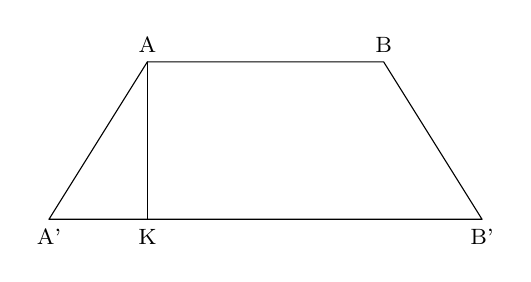
\begin{tikzpicture}[line join=round,line cap=round,>=stealth,font=\footnotesize,scale=1]
					\coordinate [label=above:A] (A) at (-6,-2);
					\coordinate [label=above:B](B) at (-3,-2);
					\coordinate [label=below:A'] (C) at (-7.25,-4);
					\coordinate [label=below:B'] (D) at (-1.75,-4);
					\coordinate [label=below:K] (K) at (-6,-4);
					\draw (A)--(B)--(D)--(C)--(A);
					\draw (A)--(K);
				\end{tikzpicture}
			}
			\item \immini{Ta có: $AC=3\sqrt{2}, A'C'=6\sqrt{2}, AA'=\sqrt{\dfrac{17}{2}}$.\\
				Dựng $AH \perp A'C'$ thì $AH \perp (A'B'C'D')$ nên đường cao của khối chóp cụt là $h = AH$.\\
				Xét $\Delta AA'H$ vuông tại $H$: \\
				$AH = \sqrt{AA'^2-AH^2}= \sqrt{\dfrac{17}{2}-\dfrac{9}{2}}=2.$
			}
			{
				\begin{tikzpicture}[line join=round,line cap=round,>=stealth,font=\footnotesize,scale=1]
					\coordinate [label=above:A] (A) at (-6,-2);
					\coordinate [label=above:C](C) at (-3,-2);
					\coordinate [label=below:A'] (B) at (-8,-4);
					\coordinate [label=below:C'] (D) at (-1,-4);
					\coordinate [label=below:H] (K) at (-6,-4);
					\draw (A)--(C)--(D)--(B)--(A);
					\draw (A)--(K);
				\end{tikzpicture}
			}
			$S_1=S_{ABCD}=3^2=9, S_2=S_{A'B'C'D'}=6^2=36, h = 2 $\\
			$\Rightarrow V_{ABCD.A'B'C'D'}=\dfrac{1}{3} \sqrt{S_1^2+S_2^2+S_1S_2}.h = \dfrac{1}{3} \sqrt{9^2+36^2+9.36}.2=2\sqrt{179} \text{ dm}^3$ .\\
			Vậy, thùng có thể đựng tối đa $2\sqrt{179}$ lít nước.
		\end{enumEX}
	}
\end{vd}



\subsubsection{Bài tập tự luận}

\begin{bt}%[1T4Y4-2]
	Hộp giấy có các mặt là hình chữ nhật ở Hình 3a được vẽ lại với các đỉnh là $A,B,C,D$, $A',B',C',D'$ như Hình 3b. Quan sát hộp giấy và chỉ ra các cặp mặt phẳng song song với nhau ở Hình 3b.\\
	\begin{center}
		\begin{minipage}[b]{0.4\textwidth}
			\includegraphics[scale=0.5]{HINHVE/CTST/CTST-4_4_1}
			\centerline{Hình 3a}
		\end{minipage}
		\begin{minipage}[b]{0.4\textwidth}
			\begin{center}
				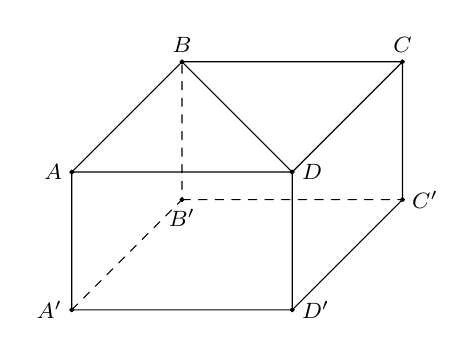
\begin{tikzpicture}[scale=0.7, font=\footnotesize, line join=round, line cap=round, >=stealth]
					\coordinate (M) at (0,0);
					\coordinate (N) at (2,2);
					\coordinate	(Q) at (6,2);
					\coordinate	(P) at (4,0);
					\coordinate (A) at (0,2.5);
					\coordinate (B) at (2,4.5);
					\coordinate	(C) at (6,4.5);
					\coordinate	(D) at (4,2.5);
					\draw[fill=black] (M) node[left]{$A'$} circle(1pt);
					\draw[fill=black] (N) node[below]{$B'$} circle(1pt);
					\draw[fill=black] (Q) node[right]{$C'$} circle(1pt);
					\draw[fill=black] (P) node[right]{$D'$} circle(1pt);
					\draw[fill=black] (A) node[left]{$A$} circle(1pt);
					\draw[fill=black] (B) node[above]{$B$} circle(1pt);
					\draw[fill=black] (C) node[above]{$C$} circle(1pt);
					\draw[fill=black] (D) node[right]{$D$} circle(1pt);
					\draw (A)--(B)--(C)--(D)--(A) (B)--(D) (A)--(M)--(P)--(D) (P)--(Q)--(C);
					\draw[dashed] (M)--(N)--(B) (N)--(Q);
				\end{tikzpicture}
			\end{center}
			\centerline{Hình 3b}
		\end{minipage}
	\end{center}
	\loigiai{
		Các cặp mặt phẳng song song với nhau ở Hình 3b là: $(ABCD)$ và $(A'B'C'D')$; $(AA'B'B)$ và $(DD'C'C)$; $(AA'D'D)$ và $(BB'C'C)$.
	}
\end{bt}

\begin{bt}%[1T4B4-7]
	Để làm một khung lồng đèn kéo quân hình lăng trụ lúc giác $ABCDEF.A'B'C'D'E'F'$, Bình gắn hai thanh tre $A_1D_1$, $F_1C_1$ song song với mặt phẳng đáy và cắt nhau tại $O_1$ (hinh bên dưới).
	\begin{center}
		\includegraphics[scale=.9]{HINHVE/CTST/CTST-4_4_2}
		\begin{tikzpicture}[scale=.5, font=\footnotesize, line join=round, line cap=round, >=stealth]
			\path
			(0,1) coordinate (A)
			(1,0) coordinate (B)
			(4,0) coordinate (C)
			(6,1) coordinate (D)
			(5,2) coordinate (E)
			(2,2) coordinate (F)
			(0,8) coordinate (A')
			(1,7) coordinate (B')
			(4,7) coordinate (C')
			(6,8) coordinate (D')
			(5,9) coordinate (E')
			(2,9) coordinate (F')
			(0,4) coordinate (A_1)
			(1,3) coordinate (B_1)
			(4,3) coordinate (C_1)
			(6,4) coordinate (D_1)
			(5,5) coordinate (E_1)
			(2,5) coordinate (F_1)
			(3,4) coordinate (O_1)
			;
			\draw (A)--(B)--(C)--(D) (A')--(B')--(C')--(D')--(E')--(F')--(A')--(A) (B)--(B') (C)--(C') (D)--(D');
			\draw[dashed] (A)--(F)--(E)--(D) (F)--(F') (E)--(E') (A_1)--(D_1) (C_1)--(F_1);
			\foreach \x/\g in{A/180, B/-120, C/-60, D/0, E/0, F/-90, A'/180, B'/50, C'/90, D'/0, E'/90, F'/90, A_1/180, C_1/0, D_1/0, F_1/150, O_1/90}
			\fill[black](\x)circle(1pt)($(\x)+(\g:3mm)$)node{$\x$};
		\end{tikzpicture}
	\end{center}
	\begin{enumerate}
		\item Xác định giao tuyến của mặt phẳng $\left(A_1D_1,F_1C_1\right)$ với các mặt bên của lăng trụ.
		\item Cho biết $A'A_1 = 6AA_1$ và $AA' = 70$ cm, tính $CC_1$ và $C_1C'$.
	\end{enumerate}
	\loigiai{
		\begin{center}
			\begin{tikzpicture}[scale=.7, font=\footnotesize, line join=round, line cap=round, >=stealth]
				\path
				(0,1) coordinate (A)
				(1,0) coordinate (B)
				(4,0) coordinate (C)
				(6,1) coordinate (D)
				(5,2) coordinate (E)
				(2,2) coordinate (F)
				(0,8) coordinate (A')
				(1,7) coordinate (B')
				(4,7) coordinate (C')
				(6,8) coordinate (D')
				(5,9) coordinate (E')
				(2,9) coordinate (F')
				(0,4) coordinate (A_1)
				(1,3) coordinate (B_1)
				(4,3) coordinate (C_1)
				(6,4) coordinate (D_1)
				(5,5) coordinate (E_1)
				(2,5) coordinate (F_1)
				(3,4) coordinate (O_1)
				;
				\draw (A)--(B)--(C)--(D) (A')--(B')--(C')--(D')--(E')--(F')--(A')--(A) (B)--(B') (C)--(C') (D)--(D');
				\draw[dashed] (A)--(F)--(E)--(D) (F)--(F') (E)--(E') (A_1)--(D_1) (C_1)--(F_1);
				\foreach \x/\g in{A/180, B/-120, C/-60, D/0, E/0, F/-90, A'/180, B'/50, C'/90, D'/0, E'/90, F'/90, A_1/180, B_1/180, C_1/0, D_1/0, E_1/0, F_1/150, O_1/90}
				\fill[black](\x)circle(1pt)($(\x)+(\g:3mm)$)node{$\x$};
			\end{tikzpicture}
		\end{center}
		\begin{enumerate}
			\item Qua $O_1$ kẻ $B_1C_1$ song song với mặt phẳng đáy như hình vẽ, khi đó ta có
			\begin{itemize}
				\item $\left(A_1D_1,F_1C_1\right)\cap\left(ABB'A'\right) = A_1B_1$.
				\item $\left(A_1D_1,F_1C_1\right)\cap\left(BCC'B'\right) = B_1C_1$.
				\item $\left(A_1D_1,F_1C_1\right)\cap\left(CDD'C'\right) = C_1D_1$.
				\item $\left(A_1D_1,F_1C_1\right)\cap\left(DEE'D'\right) = D_1E_1$.
				\item $\left(A_1D_1,F_1C_1\right)\cap\left(EFF'E'\right) = E_1F_1$.
				\item $\left(A_1D_1,F_1C_1\right)\cap\left(AFF'A'\right) = A_1F_1$.
			\end{itemize}
			\item Ta có $\heva{&A'A_1 = 6AA_1\\&A'A_1 + AA_1 = AA' = 70} \Leftrightarrow\heva{&A'A_1 = 60\\&AA_1 = 10.}$\\
			Suy ra $CC_1 = AA_1 = 10$ cm và $C_1C' = A_1A' = 60$ cm.
		\end{enumerate}
	}
\end{bt}

\begin{bt}%[1T4B4-7]
	Chỉ ra các mặt phẳng song song trong mỗi hình sau. Tìm thêm một số ví dụ khác về các mặt phẳng song song trong thực tế.
	\begin{center}
		\includegraphics[scale=.5]{HINHVE/CTST/CTST-4_4_3}
	\end{center}
	\loigiai{
		\begin{itemize}
			\item Các tấm pin năng lượng mặt trời mô phỏng hình ảnh các mặt phẳng song song.
			\item Các tấm kính ốp đối diện nhau xung quanh tòa nhà mô phỏng hình ảnh các mặt phẳng song song. 
			\item Trần nhà và sàn nhà, các bậc cầu thang bộ, từng lớp của ruộng bậc thang, ... cho ta hình ảnh của những mặt phẳng song song trong thực tế.
		\end{itemize}
	}
\end{bt}